\chapter{Was ist Reactive Programming}\label{was_ist_reactive_programming}
Ist man neu in der Domäne von reaktiver Entwicklung stellt man schnell fest, dass allerhand mögliche Definitionen und Beschreibungen findet was Reactive Programming denn zu sein scheint. Bevor jedoch hier eine Definition erläutert wird, muss zwischen unterschiedlichen Begrifflichkeiten differenziert werden: \textit{Reactive Systems, Functional Reactive Programming} und natürlich \textit{Reactive Programming}. Vorab wird jedoch ergründet worum es sich grundlegend handelt und wieso es zur heutigen Zeit von Relevanz ist, über die möglichen Verwendung von Reactive Programming zu sprechen.
\section{Was bedeutet \textit{"reactive"} im Kontext der Softwareentwicklung}
Wie die Wortherkunft verlauten lässt, wird etwas als reaktiv bezeichnet, wenn eine Reaktion durch eine vorangegangene Aktion ausgelöst wird. Bei diesen Aktionen handelt es sich meist um Veränderungen an verwendeten Daten und stattfindende Ereignisse(\textit{Events}). Eine gutes Beispiel zur Veranschaulichung ist die Benutzeroberfläche(\textit{GUI - Graphical User Interface}). Ein Benutzer bestätigt eine vorgenommene Eingabe durch das klicken eines Button innerhalb der GUI. Dieses Event sorgt dafür, dass die Applikation einen vorgegebenen Vorgang ausführt. Dieses Vorgehen sorgt in der klassischen objektorientierten Programmierweise mit sequentiellem Ablauf sowie dem imperativen Ansatz grundsätzlich für ein stetig wachsendes Maß an Komplexität. Durch die unterschiedlichen Events die innerhalb der GUI ausgelöst werden können(Mausklick, Tastendruck, usw.) ist ein klassischer imperativer sowie sequentieller Ablauf den Programmcodes nicht realistisch, da kein Entwickler weiß, in welcher Reihenfolge und zu welchem Zeitpunkt ein beziehungsweise welches Event ausgelöst wird. Somit spielt hier die \textit{Inversion of Control}\footnote{Vgl. \cite{MartinFowler.2005}, https://martinfowler.com/bliki/InversionOfControl.html.}, also das Umkehren der Kontrolle, eine große Rolle. Diese besagt, dass nicht der geschrieben Code den Ablauf beschreibt, sondern die Kontrolle bei dem Framework\footnote{In diesem Fall ein Framework für das Realisieren einer GUI. Vgl. \cite{wiki.guilist}.}, welches für die Interaktion zuständig ist, liegt, und dieses entscheidet wiederum wie und wann auf ein Event reagiert wird. Im Code spiegelt sich das dadurch wider, das mögliche Reaktionen, meist als Methoden oder Funktionen realisiert, an die mögliche eintreffenden Ereignisse gebunden werden. Dies geschieht über so genannte Event-Handler beziehungsweise Event-Listener oder über die Verwendung von Callbacks. 

\lstinputlisting[linerange={6-14}, caption={Implementierung des eigentlichen Event Handlers}, label=lst:handler]{../SystemMonitor/examples/eventhandling/Handler.java}

Im Listing \ref{lst:handler} sieht man eine Klasse welche das Event Hander Interface implementiert. Das Interface liefert eine Funktion welche überschrieben werden muss. Innerhalb dieser Methode wird die Reaktion auf das aufgetretene Event definiert, in diesem Beispiel soll in Konsole die Event-Art ausgegeben werden. In Listing \ref{lst:eventrunner} wird nun dem einzigen Element der GUI, dem Button, ein Event Handler hinzugefügt. Die Parameter besagen, dass jedes auftretenden Mouse-Event den Handler auslöst. Somit wird der Handler ein ein auftretendes Ereignis gebunden, und dir Programmablauf findet nicht mehr sequentiell statt, sondern das Framework der Oberfläche erkennt das Event und der passende Handler wird aufgerufen. Ein einem Objekt können natürliche mehrere Handler gebunden werden, die auf das gleiche oder unterschiedliche Event reagieren müssen.

\lstinputlisting[linerange={10-29}, caption={Klasse zum Anwendungsstart in welcher auch der EventHander gesetzt wird.}, label=lst:eventrunner]{../SystemMonitor/examples/eventhandling/ApplicationRunner.java}

Ein bewährtes und klassisches Vorgehen bei Anwendungsanforderungen dieser Art ist das schon 1994 von Erich Gamma und seinen Mitstreitern beschriebenes Entwurfsmuster\footnote{\cite{Gamma.2011}: Dieses Buch beschreibt viele noch heute verwendete Entwurfsmuster. Die Autoren sind in die Geschichte als die Gang Of Four (\textit{GoF}) eingegangen.}, dem \textit{Observer-Pattern}. 
Auch hier lässt sich wieder die GUI als guten Beispiel heran ziehen. Man betrachtet eine Oberfläche welche die Temperatur im Raum anzeigt, diese Oberfäche repräsentiert in Abbildung \ref{pic:observerpattern} das Subject. Die Temperatur wird als Zahl in Grad Celsius sowie graphisch in einem Balken dargestellt. Obwohl beide Elemente auf die selben Daten zugreifen, stehen programmatisch die Objekte in keine Zusammenhang. Um nun das Beobachtermuster zu implementieren, muss der sich ändernde Wert, der zum Beispiel von einem Temperatursensor gemessen wird, beobachtet werden. Deshalb werden die beiden Objekte, die Ausgabe per Zahlenwert und der graphische Balken, als Observer, in der Abbildung als ConcreteObserverA und ConcreteObserverB registriert. Dies heißt wiederum, dass die beiden Observer die \textit{register()}-Methode des Subjects aufrufen und somit in die Observer-Liste dieses Subjects aufgenommen werden. Ändert sich nun zum Beispiel die Temperatur wird die \textit{notifyObservers()}-Methode aufgerufen, was heißt, dass über die Liste der Observer iteriert wird und die \textit{update()}-Methode jedes Observers aufgerufen wird.
\begin{figure}
	\centering
	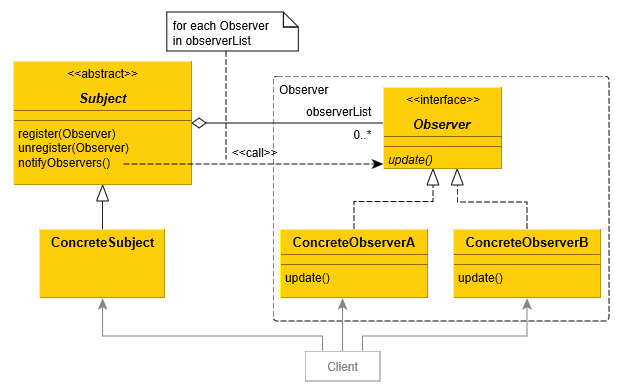
\includegraphics[width=1\textwidth]{Abb/observerpattern}
	\caption{Schematischer Aufbau eines Observer Patterns. Quelle: https://www.philipphauer.de/study/se/design-pattern/observer.php}
	\label{pic:observerpattern}
\end{figure}
Diese Methoden können nach dem \textit{Push} oder \textit{Pull} Verfahren implementiert werden. Bei Verwendung des Push-Modells wird dem Observer der Wert des geänderten Parameters direkt mitgeteilt. Das Pull-Modell verfolgt den Ansatz, dass der Observer eine Information erhält, dass sich Werte geändert haben, muss jedoch über die Getter-Methoden die für ihn relevanten Wert aktiv nachfragen. Je nach Vorgehen ergeben sich Vor- und Nachteile. Der Push-Ansatz steht eher für lose Kopplung, da der Observer keine Details des Subject wissen muss. Jedoch sinkt dadurch die Flexibilität, da Observer Interfaces exakter beschrieben werden müssen, damit das Subject weiß, welche Information weiter gereicht werden sollen. Die Kopplung im Vergleich zum Pull-Ansatz ist nicht wirklich lose, da jeder Beobachter wissen muss, welche Daten das observierte Objekt repräsentiert und wie auf diese Daten zugegriffen werden kann. Jedoch findet sich hier die Flexibilität wieder, da jeder Beobachter wenn er Information braucht, exakt diese Daten abrufen kann und sich nicht auf die korrekte Datenverteilung des Subjects verlassen muss. 
\subsection{Differenzierung zwischen Reactive Proramming und Reactive Systems}
Das zuvor angesprochene Verhalten bezieht sich nur auf ein Beispiel. Wie jedoch wirkt es sich aus, wenn eine komplette Anwendung unter Verwendung dieses Stils entwickelt wird? Wie verhält es sich weiter wenn mehrere Teile reaktiv funktionieren und kommunizieren sollen? Der grundlegende Gedanke reaktiver Systeme wurde schon im Jahre 1985 in einem Paper von D. Harel und A. Pnueli beschrieben\footnote{\cite{Harel1985}. Wohl das erste Schriftstück zur Behandlung von reaktiven Systemen}. Zur heutigen Zeit jedoch bezieht man sich bei Richtlinien zur Gestaltung reaktiver Anwendungen eher auf das Reactive Manifesto\footnote{\cite{Boner.2014}. Das Manifest wird von über 19.000 Menschen unterstützt und gilt als fester Bestandteil der Reactive Development Gemeinschaft und wird auch mit Unterstützung derer immer genauer spezifiziert.}. Laut Jonas Bonér und den vielen Unterstützern sind vier Bestandteile essentiell, damit eine Anwendung die Anforderung erfüllt um sich reaktiv zu verhalten. Die Ansicht des Manifest stützt sich auf einen Architektur- beziehungsweise Designstil und soll als Grundlage zur Entwicklung reaktiver Systeme dienen. Die folgenden Erklärungen sind dem Manifest entnommen und sollen einen Verständnis zu den vier Eigenschaften bieten wie sie auch in Abbildung \ref{pic:manifest4} aufgezeigt werden. Wie in diesem beschrieben sind Reaktive Systeme:
\begin{figure}
	\centering
	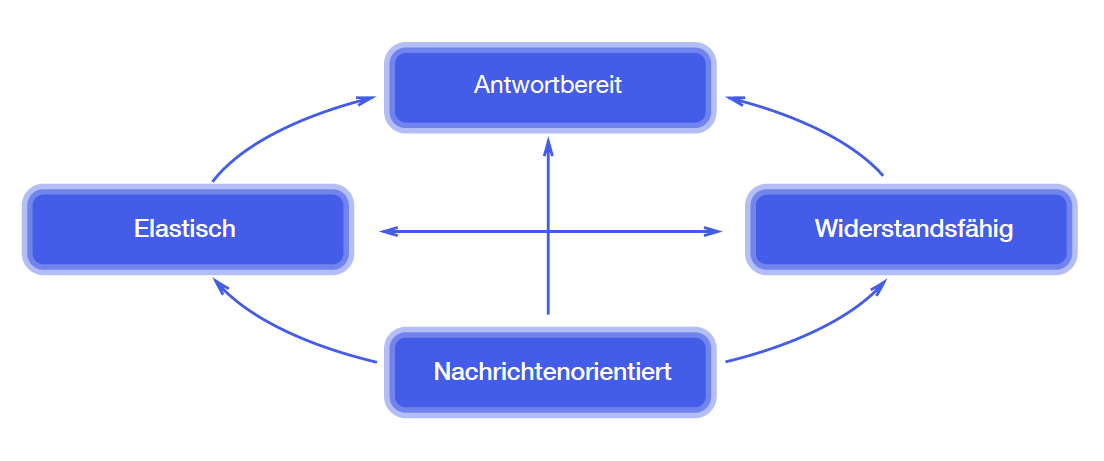
\includegraphics[width=1\textwidth]{Abb/manifest4achsen.PNG}
	\caption{Die vier relevanten Bestandteile für ein reaktives System. Quelle: http://www.reactivemanifesto.org/de}
	\label{pic:manifest4}
\end{figure}
\begin{itemize}
	\item \textbf{Antwortbereit (engl. responsive):}\\ Ein System muss immer zeitgerecht antworten. Die Antwortbereitschaft ist die Grundlage für die Benutzbarkeit besagten Systems. Ebenso wird um eine Fehlerbehandlung durchführen zu können eine geregelte Antwortbereitschaft vorausgesetzt.
	\item \textbf{Widerstandsfähig (engl. resilient):}\\ Ein System muss auch bei Ausfällen die Antwortbereitschaft aufrecht erhalten. Die wird durch Replikation der Funktionalität, der Isolation von Komponenten sowie dem Delegieren von Verantwortung erzielt. 
	\item \textbf{Elastisch (engl. elastic):}\\ Das System muss bei sich ändernden Lasten die Funktionalität und Antwortbereitschaft aufrecht erhalten. Ressourcen müssen den auftretenden Lasten, ob steigend oder sinken, angepasst werden können.Ebenso müssen Engpässe innerhalb des Systems unterbunden werden um die Elastizität zu bewahren.
	\item \textbf{Nachrichtenorientiert (engl. message driven):}\\ Ein loses System soll zur Kommunikation zwischen den Komponenten auf asynchrone, ortsunabhängige Nachrichtenübermittlung zurück greifen. Somit ist nicht relevant auf welchen Rechner die einzelnen Komponenten ausgeführt werden, wodurch wiederum eine gute Skalierbarkeit entsteht.
\end{itemize}
Das Manifest erwähnt jedoch in keinster Weise den Zusammenhang von Systemen zum Reactive Programming. Auch aus diesem Grund hat Jonas Bonér einen weiteren Artikel\footnote{\cite{Boner.}.} verfasst, der sich dieser Thematik annimmt. Die grundlegenden Unterschiede wurde in dem Artikel wie folgt zusammengefasst:
\begin{itemize}
	\item Reactive Programming ist eine Teilmenge von reaktiven Systemen auf Implementierungsebene
	\item Reactive Programming liefert Leistung und effektive Ressourcennutzung auf Komponentenebene, speziell für Softwareentwickler
	\item Reaktive Systeme hingegen bieten Robustheit und Elastizität auf Systemebene zur Gestaltung von Cloud-kompatiblen oder verteilten Anwendungen, speziell für Softwarearchitekten oder DevOps
	\item Es ist von großem Vorteil Reactive Programming innerhalb der Bestandteile von reaktiven Systemen zu verwenden
	\item Es is ebenso von Vorteil reaktive Systeme zur Interaktion zwischen reaktiv programmierten Komponenten zu verwenden
\end{itemize}
Wie aus diesen Punkten klar wird, liegt also der genaue Unterschied zwischen Reactive Programming und Reactive Systems darin, aus welcher Perspektive die Betrachtung stattfindet. Architektonisch wird von Systemen gesprochen, die innerhalb und zur Interaktion mit anderen reaktiv reagiert. Betrachtet man das Ganze aus Entwicklersicht in Bezug auf eine Komponente, kann diese unter Zuhilfenahme von Reactive Programming für ein asynchrones, paralleles Verhalten entwickelt werden. Wie Jonas Bonér schon schreibt, ist das Zusammenspiel beider sehr oft hilfreich um das gewünschte Ziel zu erreichen. Ein weiterer wichtiger Punkt ist die Unterscheidung von \textit{ereignisorientiert} zu \textit{nachrichtenorientiert}. Nachrichten werden auf Systemebene genutzt. im Gegensatz zu Ereignissen sind Nachrichten klar an einen Empfänger adressiert. Ereignisse treten auf und müssen beobachtet werden um das gewünschte Resultat zu erzielen. Nachrichten sind somit gut geeignet bekannte Empfänger in einem verteilten System, zum Beispiel über das Netzwerk, zu kontaktieren. Innerhalb der Komponente besteht die Funktion (man denke hier wieder an die Nutzeroberfläche) oft aus der Reaktion auf Ereignisse unterschiedlicher Art die direkt in der Komponente verarbeitet werden sollen. Somit herrscht hier ein ereignisgetriebenes  Verhalten. 

\section{Reactive Programming vs. Functional Reactive Programming}
Auf der Suche nach einer Definition zu Reactive Programming stößt man oft auf es Begriff Functional Reactive Programming. Teilweise werden die Begriffe sogar synonym verwendet\footnote{Vgl.: \cite{Nurkiewicz.2017}, Seite 2.}. Grundlegend betrachtet man bei den bekannten Programmierparadigmen zwischen imperativen und deklarativen Paradigmen, wobei zum Beispiel die objektorientierte Programmierung im imperativen und funktionale Programmierung im deklarativen Bereich angesiedelt wird. Funktionale Programmierung zeichnet vor allem die Nutzung des Lambda-Kalküls\footnote{Vgl. \cite{lambda}, Wiki Eintrag zum Lambda-Kalkül} aus. Ein Lambda Ausdruck wird in der Mathematik wie folgt dargestellt:
\begin{displaymath}
	\lambda x.x+2
\end{displaymath}
Dieser Ausdruck besagt, dass jeder Wert $x$ auf $x+2$ abgebildet wird.
 Statt Rechenanweisungen werden Programme als Menge von Definitionen beschrieben, die mathematisch eine Abbildung von Eingabedaten auf Ausgabedaten darstellt und gleichzeitig selbst aus Funktionsaufrufen zusammengesetzt sind \footnote{Vgl. \cite{funktioprogrammierung}, Wiki Eintrag zur funktionalen Programmierung.}. Wird eine funktionale Programmiersprache nun um den relevanten Faktor Zeit erweitert kann ein reaktives Verhalten beschrieben werden. Diese Art der Realisierung nennt man \textit{Functional Reactive Programming}\footnote{Vgl. \cite{frp.haskell}, Haskell Wiki zu Functional Reactive Programming}. Dieser Zeitfaktor zeigt sich im Funktionalen in der kontinuierlichen Wertänderung im Laufe der Zeit. Somit kann das Functional Reactive Programming als Teilmenge des Paradigma der reaktiven Programmierung angesehen werden. Die Verwechslung der Begriffe entsteht wenn man sich zum Beispiel Java 8 anschaut. Mit Java 8 nahm die Klasse der Funktionen sowie die Lambda-Ausdrücke Einzug in die objektorientierte Programmiersprache Java. In Java-Code werden Lambda-Ausdrücke wie folgt dargestellt:
 \begin{lstlisting}[language=java, caption={Lambda Beispiel in Java}, label=lst:LambdaJava, frame=single]
 	List< Integer > list = Arrays.asList( 1, 2, 3, 4, 5 );
 	list.forEach( element -> System.out.println( "Number" + element ) );
 	 \end{lstlisting}
In \ref{lst:LambdaJava} wird jedes der Listenelemente wird auf die Konsolenausgabe mit konkateniertem String abgebildet. Dadurch wird ein ähnliches Verhalten der funktionalen Programmierung reproduziert. Somit kann innerhalb von Java reaktiv unter Zuhilfenahme von funktionalen Methodiken entwickelt werden. Der Unterschied findet sich also genau an der Stelle, dass funktionale Eigenschaften zwar in Java vorhanden sind, dadurch Java allerdings nicht als funktionale Programmiersprache verstanden werden kann, denn auch innerhalb der Objektorientierung kann auf dem imperativen Weg ein reaktives Verhalten entwickelt werden. Faktor Zeit wird im reaktiven Programmieren eher darin reflektiert, dass konkrete Werte im Laufe der Zeit gesendet werden. Reactive Programming kann somit als eine Abstraktion gesehen werden, die sich über die Vorhandenen Paradigmen erstreckt und je nach Situation und Anwendungsbereich auf andere Programmierstile zurück greift. 

\section{Wie wird Reactive Programming realisiert?}
Es wurde berichtet was allgemein unter einem reaktiven Verhalten verstanden wird. Ebenso wurde die Begrifflichkeiten und Zusammenhängen zwischen Reactive Programming, Reactive Systems und Functional Reactive Programming erläutert. Es stellt sich jedoch noch die Frage wieso aktuell die Reaktivität von Applikation stark gefordert wird und wie eine Umsetzung davon aussieht. Durch große Datenraten, Datenmengen und vielen vernetzten Geräte und Dienste die zur heutigen Zeit in Umlauf sind, entstehen viele Informationen die verarbeitet werden können beziehungsweise müssen. Durch die vielen Berechnungen und Verarbeitungsschritte die dafür nötig sind, spielt hier das Gesetz von Amdahl eine große Rolle\footnote{Vgl. \cite{Amdahl.}. Es handelt sich um einen Reprint in der IEEE SSCS News. Auf diesem von Amdahl verfassten Original resultiert das gleichnamige Gesetz.}. Dieses besagt, dass nie alle Teile eines Programms parallel ausgeführt werden können. Somit lohnt es sich, denn Ablauf in einen sequentiellen und einen parallelen Teil zu zerlegen. Die Blockade die somit noch bleibt, sind die Programmteile die sequentiell abgearbeitet werden müssen und nicht weiter optmiert werden können. Reactive Programming versucht nun eine Lösung abzubilden die den Ablauf innerhalb des parallelen Teils vereinfacht und beschleunigt um eine möglichst geringe Latenz und große Flexibilität und Reaktionsfreudigkeit eines Programms widerzuspiegeln. Ein Ansatz diese Lösung zu realisieren ist die Verwendung von Streams. Die Stream-Api wurde wie die Lambda-Funktionalität mit Java 8 eingeführt. Sich veränderte oder neue Daten werden als Ströme betrachtet, die unter Beobachtung stehen und Änderungen sowie Bearbeitung der Daten asynchron und parallel zu den anderen Funktionen einer Anwendung ausgeführt werden können. Damit dieses Verfahren der Datenverarbeitung funktioniert, sind einige Konzepte zu beachten.
\subsection{Streams}
Das Konzept der Streams stellt eine Abstraktion für Folgen von Bearbeitungsschritten auf Daten dar\footnote{Vgl. \cite{Inden.2015}, Seite 42.}. Streams erinnern an Collections sind jedoch nur einmal traversierbar und nehmen keine direkten Speicherung der Daten vor. Collections können auch als Streams respräsentiert werden. Nahe liegt die verbreitete Analogie der Fließbandverarbeitung. Man hat eine Menge von Objekten die nacheinander gewissen Operationen unterzogen werden. Diese wird einmalig durchgeführt und die Zwischenergebnisse bleiben nicht vorhanden. In Listing \ref{lst:streamsandbulk} sieht man, dass mit dem Methodenaufruf \textit{stream()} auf der Collection ein Stream parametrisiert auf den selben Datentyp wie die Collection erstellt werden kann. Es findet keine Änderung an den einzelnen Elemente statt, denn er werden nur Kopien weiter gereicht.
\lstinputlisting[linerange={7-14}, caption={Beispiel Erstellung, Verarbeitung und Ergebnisermittlung von Streams.}, label=lst:streamsandbulk]{../SystemMonitor/examples/streamsandbulk/StreamsAndBulk.java}
\subsection{Bulk Operations}
Diese Operationen gelten als funktional in sind seit Java 8 auf Collections sowie Streams anwendbar. Diese Operation müssen nicht separat implementiert werden und können direkt auf Collections oder Streams ausgeführt werden. Jedoch sind nicht zu beiden Arten die exakt gleichen Operation verfügbar. Somit kann durch eine Operation zum Beispiel eine Veränderung an jedem Objekt einer Liste ausgeführt werden, oder eben auf jedem Objekt welches einen Stream durchquert. Die Operation können verkettet werden. Zu beachtet ist, dass jede Operation auf einer Kopie des eigentlichen Objekts ausgeführt wird, also bleibt zum Beispiel die Liste unverändert wenn man solch eine Massenoperation auf die Elemente der Liste ausführt. Als Ergebnis wird eine modifizierte Kopie der ursprünglichen Liste geliefert. Auch bei einer Verkettung wird immer nur eine Kopie des Eingangsobjekts modifiziert und weiter gereicht. Erwähnung sollte noch die unterschiedliche Art von Operation finden. Es wird zwischen drei Arten von Operationen unterschieden: \textit{Erzeugung}, \textit{Berechnung} und \textit{Ergebnisermittlung}\footnote{Vgl.: \cite{Inden.2015}, Seite 42f.} die sich wie folgt abbilden lassen: 
\begin{displaymath}
	\underbrace{Quelle \Rightarrow STREAM}_{Erstellung} \Rightarrow \underbrace{OP_{1} \Rightarrow OP_{2} \Rightarrow ... \Rightarrow OP_{n}}_{Berechnung} \Rightarrow \underbrace{Ergebnis}_{Ergebnisermittlung}
\end{displaymath}
Bei der Erzeugung wird von der Änderung der Datenrepräsentation von einem Datentyp einer Collection oder eines Arrays in einen Stream gesprochen. Java bietet hierfür für jeweils Arrays oder Collections Methoden an. Resultieren erhält man einen Stream. Eine Reihe von Berechnungen kann nun verketten stattfinden, zum Beispiel eine direkte Manipulation oder Filterung nach Kriterien. Sind die Berechnungen abgeschlossen wird das Ergebnis zum Beispiel auf der Konsole ausgegeben oder in einem Datentyp gespeichert. Konkret ist der Ablauf in Listing \ref{lst:streamsandbulk} zu sehen. Wie vorhin schon erwähnt wird via Methodenaufruf eine Stream-Repräsentation der Collection geschaffen. Die Berechnung beziehungsweise Bearbeitung finden in der Konkatenation der Operation \textit{map()} und \textit{filter()} statt. Zuerst wird eine Kopie jeden Strings in Großbuchstaben transformiert, anschließend wird gefiltert ob der String ein \textit{\"L\"} enthält. Die Ergebnisermittlung findet in der \textit{forEach()}-Methode statt, da hier jedes Element das nach dem filtern noch übrig ist auf die Konsole geschrieben wird. Es können noch beliebig viele Stream-Objekte von einer Collection erstellt werden, ebenso kann beliebig oft durch einen Stream durch gegangen werden. Dies ist möglich das nie eine direkte Änderung vorgenommen wird, sondern wie erwähnt immer nur Kopien weiter gegeben werden.
\subsection{Back Pressure}
Man nehme an, zwei Streams stehen in Verbindung zueinander. Die Bearbeitung der einzelnen Ströme finden asynchron und parallel statt, so wie es bei der reaktiven Programmierung beabsichtigt wird. Der eine Stream führt nun eine kurze Überprüfung durch der zweite führt eine Berechnung durch. Nach dieser Berechnung soll eine Verknüpfung mit dem nächsten Objekt des ersten Streams stattfinden, jedoch ist die Überprüfung doppelt so schnell. Dadurch entsteht ein Rückstau innerhalb des ersten Streams. Je nach Implementierung werden alle Elemente auf Seiten des Verarbeitenden gepuffert\footnote{Zum Beispiel bei der Observable-Klasse des RxJava2 Frameworks}. Dieses theoretische Beispiel zeigt, dass es bei der Arbeit mit vielen asynchronen und parallelen Operationen als sehr wichtig gilt, jede Interaktion zwischen zweier solcher Programmelemente genau zu kalkulieren. Findet dies nicht statt, kann zum Beispiel ein hoher Ressourcenverbrauch oder ein Programmabsturz durch eine \textit{OutOfMemoryError} die Folge sein. Um dies zu verhindern muss diese Art von Fehler vorbeugend behandelt werden um Schlimmeres zu verhindern. Eine Möglichkeit wäre zum Beispiel das Setzt einer festen Puffergröße und beim Erreichen dieser das Werfen einer \textit{MissingBackpressureException}\footnote{So wird es in RxJava2 gehandhabt, siehe: http://reactivex.io/RxJava/2.x/javadoc/}.
\section{Reactive Streams}
Festhalten lässt sich somit, dass die Verarbeitung von asynchronen, parallele Streams die Reaktivität generiert. Nach dem anfangs erwähnten Observer Pattern werden die Streams observiert und die Daten werden den Observern publiziert. In der Welt der JVM wurde die Initiative der \textit{Reactive Streams}\footnote{\cite{reactivestreams}} geschaffen, um einen Standard für die Verarbeitung von asynchroner Streamverarbeitung mit nicht blockierendem Back Pressure zu etablieren. Das zu bewältigenden Problem ist die unterschiedliche Implementierung der bereits existierenden reaktiven Frameworks. Somit soll eine Kompatibilität von reaktiven Komponenten untereinander gesichert werden, auch wenn besagte Komponenten auf unterschiedliche Frameworks basieren. Viele Entwicklerteams von reaktiven Frameworks haben sich mittlerweile dieser Initiative angeschlossen und die Schnittstellen soweit angepasst, dass diese Kompatibilität gewährleistet werden kann\footnote{\cite{rs.implementations}. Auflistung der Frameworks die sich an die Vorgaben der Reactive Streams Initiative binden}. Einige der hier aufgeführten Frameworks werden in folgendem Abschnitt noch genauer beschrieben. Mit Java 9 wird in der sogenannten \textit{Flow API}\footnote{\cite{fl.apidoc}. Aktuelle Apidoc der Flow-API von Java 9} eine Implementierung nach den \textit{Reactive Streams}-Kriterien geliefert. Ein Anwendungsbeispiel wird von der offiziellen Java-Community bereits zur Verfügung gestellt\footnote{\cite{flowex}. Beispiel der Flow-API unter Berücksichtigung der Reactive Streams Initiative}.  
\section{Überblick über bekannte Frameworks und ihre Eigenschaften}
Die Welt der Softwareentwicklung bietet viele unterschiedliche Programmiersprachen für unterschiedliche Anwendungsfelder. Da es den Umfang dieser Arbeit überschreiten würde sich mit allen vorhandenen Frameworks zu den jeweiligen Sprachen zu befassen, wird auch in diesem Abschnitt hauptsächlich die Vielfalt innerhalb des Java Universums behandelt. Insbesondere die Reactor Bibliothek, das Akka Toolkit und die ReactiveX API, speziell RxJava.
\subsection{ReactiveX}
ReactiveX ist ein Open Source Projekt und vereint reaktive Bibliotheken für viele Sprachen und Frameworks unter einem Dach. Die Bibliotheken halten sich an den gleichen Aufbau und Benennung um eine gewisse Konsistenz zu erschaffen. Die erste dieser Bibliotheken wurde unter Leitung von Eric Meijer\footnote{Erik Meijer gilt als Begründer des Reactive Extensions. https://www.linkedin.com/in/erikmeijer1/} bei Microsoft entwickelt und nennt sich Rx.NET, als Erweiterung zum .NET Framework von Microsoft. Das Kürzel \textit{Rx} steht für Reactive Extentions, also reaktive Erweiterung. Folgend wurde von Ben Christensen und Jafar Husain als Entwickler bei Netflix die Erweiterung für Java geschrieben und auf GitHub veröffentlicht. Es folgten viele weitere Implementierungen für zum Beispiel Ruby, Python oder JavaScript. Vorteil von diesen Erweiterung ist die Unabhängigkeit. Somit ist die Bibliothek sehr klein bringt jedoch die nötigen Eigenschaften mit, um asynchrone und nicht blockierende Anwendungen zu entwickeln. ReaktiveX sagt über sich, dass die besten Ideen des Beobachtermuster, des Iteratormusters sowie der funktionalen Programmierung hinter ihrer Art der Implementierung steckt. Die Schon in Java vorhandenen Klassen wurden überlagert und für ein reaktives Verhalten gerüstet. Aktuell wird RxJava als Version 1 und Version 2 entwickelt. In Version 2 wurden Änderungen vorgenommen um den Vorgaben der Reactive Streams Initiative zu genügen. Da es sich nicht nur um eine Erweiterung sondern um eine Neuentwicklung parallel zu Version 1 handelt, sind im Moment beide Versionen im Entwicklungsstatus. RxJava2 wird in dieser Arbeit als Referenzbibliothek\footnote{In der Readme des offiziellen Repos (Siehe \cite{rx.repo}) wird März 2018 schon als Entwicklungsende publiziert. Somit wird in dieser Arbeit auf die zweite Version gesetzt.} verwendet, daher folgt eine genau Beschreibung in einem weiteren Kapitel. Somit wird auf ein Beispiel in diesem Abschnitt verzichtet.
\subsection{Akka}
Akka bezeichnet sich selbst als Toolkit und nicht als Framework. Es kann wie jede beliebige Bibliothek in ein Java Projekt eingebunden werden. Jedoch ist diese Werkzeugkiste etwas umfangreicher als die Erweiterungen von ReactiveX. Entscheidend ist hier das relevante Modul der \textit{Akka Streams}. Spezielle das von Akka umgesetzt Actor-Modell spielt hier eine Rolle. \footnote{Beschreibung actor Modell, am besten mit Code beispiel}. Akka versucht mit seinem Vorgehen die Prinzipien des Reaktiven Manifest und auch der Reactive Stream Initiative umzusetzen.
\subsection{Reactor}
Reactor ist der ReactiveX Erweiterung sehr ähnlich. Die API ist bis auf ein paar Gemeinsamkeiten anders benannt, jedoch ist die Funktionalität fast deckungsgleich. Dies kommt daher, dass die Codebasen von beiden Projekten praktisch identisch sind\footnote{\cite{Karnok.2016}. Dávid Karnok, Projektleiter RxJava2 und Unterstützer von Reactor.} Beide Projekte arbeiten stark zusammen und beide haben schon von den jeweils anderen Implementierungen übernommen. Reactor existiert jedoch nur in der Java Welt und wird in ersten Sinne von Pivotal entwickelt. Dadurch ergibt sich auch die Nutzung in der neuesten Version des Webentwicklungs-Frameworks Spring 5. Die Reactive Bibliothek wird ab Version 5 direkt mit Spring ausgeliefert und soll eine reaktive Reaktion für REST-API's ermöglichen und vereinfachen. 
\subsubsection{Framework für JavaFX - RxJavaFX}
Einführung und Eigenschaften erläutern
\section{Testen von reaktivem Code mit dem JUnit Framework}
Noch nichts genaues. Muss noch geschaut werden wie die Funktionalität von JUnit RP abdeckt.